In this section, we compare the performance of LP-RFFs with FP-RFFs, circulant FP-RFFs, and the \Nystrom method, on the TIMIT, YearPred, CovType, and Census datasets, showing that we can attain compression ratios of at least \todo{4x} relative to these methods, without hurting generalization performance. We then perform a more careful analysis of these results, by measuring the correlation between the $\lambda$-spectral distance $D_{\lambda}(K,\tK)$, and the generalization performance when using $\tK$. We show on both the Census regression task, as well as on a sub-sampled version of the CovType classification task, that this correlation is very strong \avner{Compute actual correlation, and compare to spectral/Frob norm} across all the kernel approximations methods we used. 
We note that in practice, in order to avoid the risk of numerical precision issues (kernel ridge regression requires matrix inversion), we do all our full-precision experiments in 64 bits---however, we report memory utilization as if we used 32 bits, to avoid inflating the relative gains of our method over the full precision approaches.


For all our experiments, we use the Gaussian kernel with the kernel width value recommended by~\citet{may2017}, and compute the memory utilization as described in Section~\ref{subsec:memory_utils}. To evaluate the performance of these kernel models, we measure the classification error for classification tasks, and mean squared error (MSE) for regression tasks ($\frac{1}{n}\sum_{i=1}^n (f_{\tK}(x_i) - y_i)^2$), on the heldout set. We include details for the datasets in Table \ref{tab:datasets} \jian{include Table in main text if have space}. For more details on our experimental protocol and hyperparameter choices, please refer to Appendix~\ref{sec:exp_details}.

\subsection{Empirical evaluation of LP-RFFs}
We compare the generalization performance of LP-RFFs to full-precision RFFs, circulant RFFs, and \Nystrom features, across four datasets, for various memory budgets.  We sweep the following hyperparameters: For LP-RFFs, we choose the precision $b \in \{1,2,4,8,16\}$. For \Nystrom, we use $m \in \{1250, 2500, 5000, 10000, 20000\}$.  For the RFF-based approximations, we use $m\in \{1250, 2500, 5000, 10000, 20000, 50000, 100000, 200000, 400000\}$.  We choose these limits differently because $\num[group-separator={,}]{20000}$ \Nystrom features have roughly the same memory footprint as $\num[group-separator={,}]{400000}$ FP-RFFs. We avoid the prohibitively large computational expense of performing a grid search to tune the initial learning rate, the regularizer, the learning rate decay, and the number of training epochs, by using the following early-stopping protocol \citep{zhang2005boosting,wei2017early}: at the end of each epoch, we decay the learning rate in half if the heldout performance is less than $1\%$ better relative to the previous best model, using MSE for regression and cross entropy for classification. Furthermore, if the model performs \textit{worse} than the previous best, we revert the model. The training terminates after the learning rate has been decayed 10 times. We use a single initial learning rate per dataset across all experiments, which we tune via grid search using $20\text{k}$ \Nystrom features. We choose to use \Nystrom features to tune the initial learning rate in order to avoid biasing the results in favor of RFF-based approximation approaches. 

In Figure \ref{fig:generalization_col}, we plot the generalization performance for all these experiments, as a function of the amount of memory used, as well as the number of features $m$. We show across all four datasets that LP-RFFs show systematically better generalization performance than the full precision baselines under different memory budget. Importantly, we can observe that the \Nystrom method has observably better generalization performance than LP-RFF and FP-RFF-based baselines under the same number of features. However, when we instead consider performance as a function of memory utilization, the opposite it true, with the RFF-based methods demonstrating superior generalization performance. This observation further validates the practical importance of comparing kernel approximation methods under memory budgets.

In Table~\ref{fig:mem_saving} we present the compression ratios we can achieve with LP-RFF, relative to the baselines, while still attaining generalization performance within $1e^{-4}$ of the full-precision baseline.  We measure this as follows:  For each baseline (FP-RFF, circulant FP-RFF, \Nystrom), we find the best performing (as well as median) model.  We then find the smallest LP-RFF model which attains within $1e^{-4}$ relative performance to this baseline.  We report the ratio of the memory used by the baseline, relative to the memory used by the LP-RFF model.  We compute this ratio across three independent runs using different random seeds, and report the average.  We can see that LP-RFFs demonstrate significant memory saving over FP-RFFs and circulant FP-RFFs, showing 2.8x-10.0x and 3.9x-30.7x compression ratios respectively. On the TIMIT dataset, there are 147 classes, and thus the full-precision learned parameters occupy a large portion of the total memory across all methods. Nonetheless, even though these LP-RFF experiments only quantize the feature mini-batches, they still attain 5.1x and 3.9x compression ratios relative to FP-RFF and circulant FP-RFF.  We shown in Section \ref{sec:lptrain} that we can improve these ratios further on TIMIT by using a low-precision model.

\begin{figure}
	\centering
	\begin{tabular}{c@{\hskip 0in}c@{\hskip 0in}c@{\hskip 0in}c}
		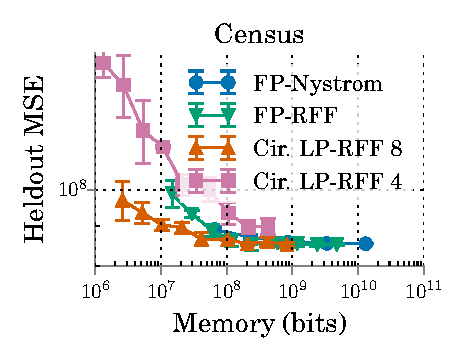
\includegraphics[width=0.3\linewidth]{figures/census_MSE_vs_n_memory.pdf} &
		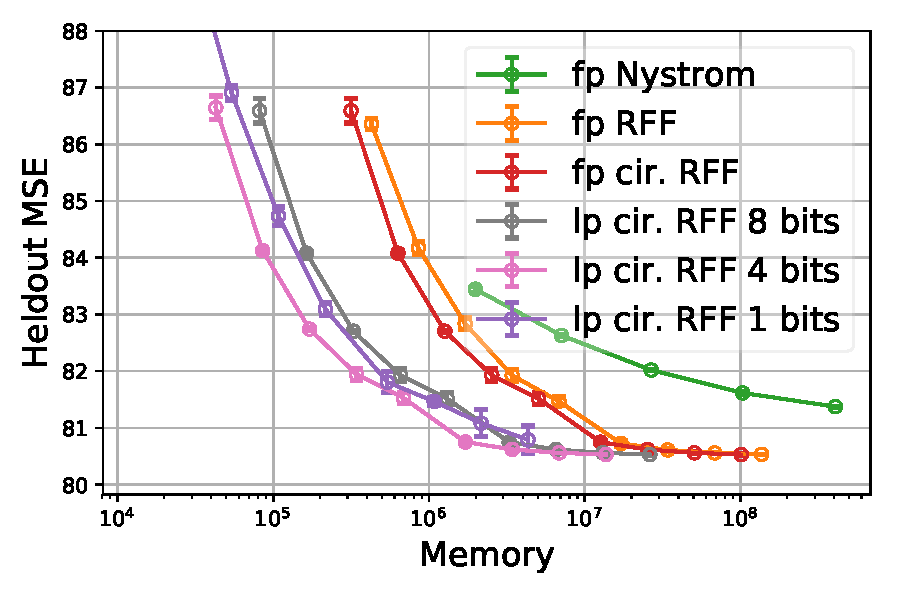
\includegraphics[width=0.3\linewidth]{figures/yearpred_MSE_vs_n_memory.pdf} &
		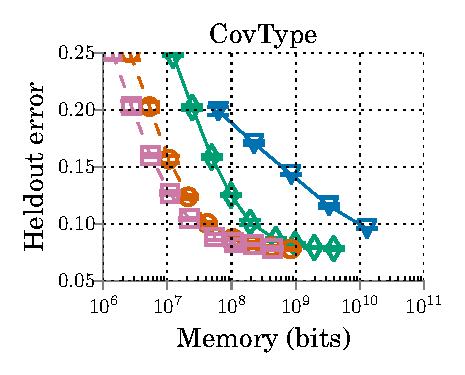
\includegraphics[width=0.3\linewidth]{figures/covtype_error_vs_n_memory.pdf} &
		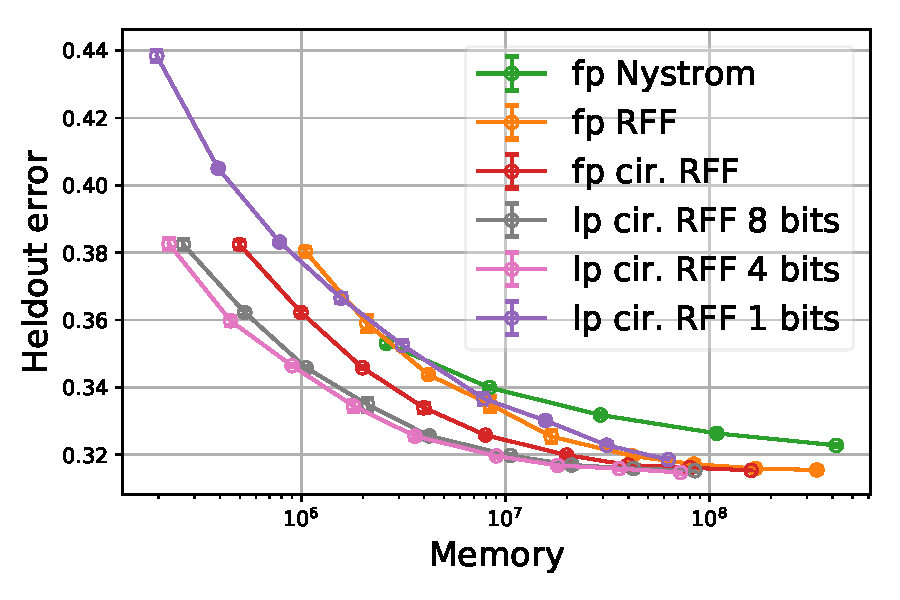
\includegraphics[width=0.3\linewidth]{figures/timit_error_vs_n_memory.pdf} \\
		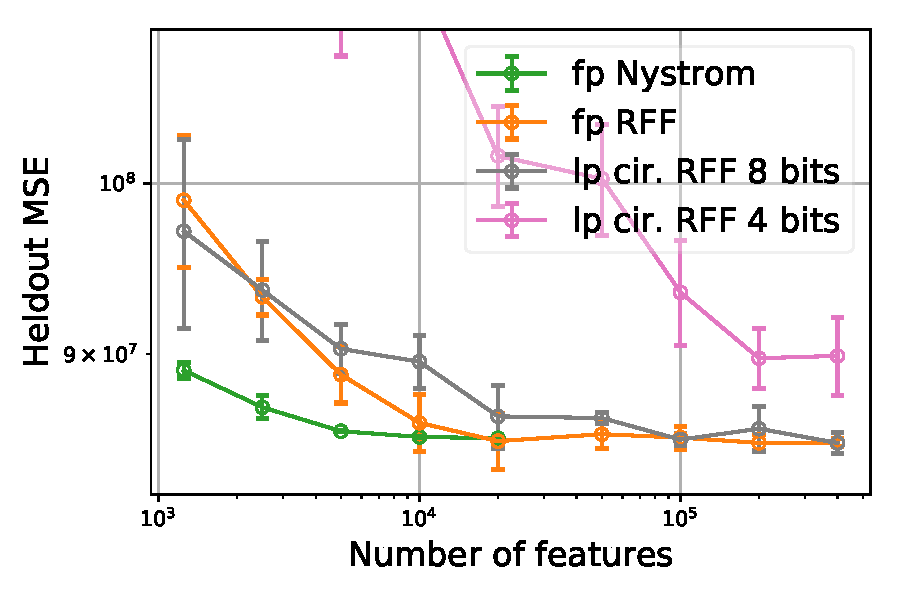
\includegraphics[width=0.3\linewidth]{figures/census_MSE_vs_n_feat.pdf} &
		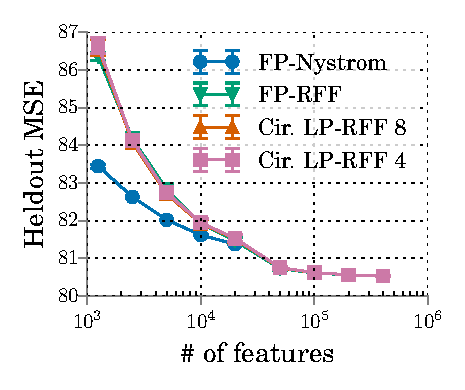
\includegraphics[width=0.3\linewidth]{figures/yearpred_MSE_vs_n_feat.pdf} &
		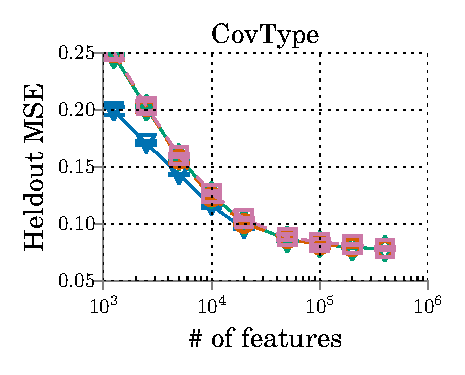
\includegraphics[width=0.3\linewidth]{figures/covtype_error_vs_n_feat.pdf} &
		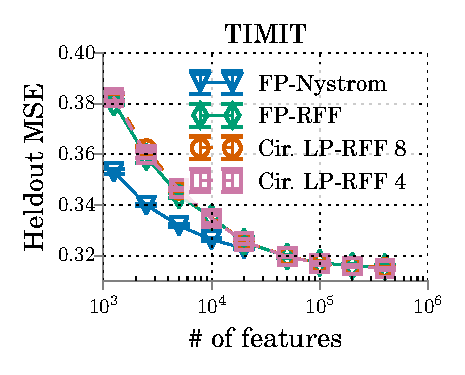
\includegraphics[width=0.3\linewidth]{figures/timit_error_vs_n_feat.pdf} \\
		(a) Census & (b) YearPred & (c) Covtype & (d) TIMIT \\
	\end{tabular}
	\caption{Generalization performance of low precision RFF, full precision RFF and \Nystrom with respect to number of features and memory budgets. Across the 4 datasets, LP RFFs demonstrate better generalization performance than full precision baselines under memory budget. Noticeably, the comparison of different methods on generalization performance behaves differently under memory budget and under number off features. E.g., \Nystrom shows better generalization performance than RFF based approach with the same number of features. However, \Nystrom can be significantly worse under memory budgets.}
	\label{fig:generalization_col}
\end{figure}

%% version with out model memory
%\begin{table}
%	\centering
%	\begin{tabular}{c c c c}
%		\hline
%		& FP RFF & FP circulant RFF & \Nystrom \\
%		\hline
%		\hline
%		Census & 5.56x & 30.32x & 122.52x \\
%		YearPred & 19.35x & 14.30x & 829.15x \\ 
%		Covtype & 9.17x & 7.57x & 460.80x \\ 
%		TIMIT & 70.42x & 25.68x & 843.41x \\ 
%		\hline
%	\end{tabular}
%	\caption{The memory savings from LP RFF to achieve within $1e^{-4}$ relative difference from the best generalization performance of baselines. We measure heldout L2 loss and heldout accuracy as the generalization performance respectively for regression and classification problems.}
%	\label{fig:mem_saving}
%\end{table}

% version with model memory
\begin{table}
	\centering
	\begin{tabular}{c c c c}
		\hline
		& FP RFF (best/median) & FP circulant RFF (best/median) & \Nystrom (best/median) \\
		\hline
		\hline
%		Census & 2.8x / 1.13x & 30.7x / 7.7x & 62.2x / 4.09x \\
%		YearPred & 10.0x / 7.3x & 14.7x / 10.8x & 436.9x / 78.0x \\ 
%		Covtype & 4.6x / 4.6x & 7.6x / 7.6x & 230.4x / 75.3x \\ 
%		TIMIT & 5.1x / 2.0x & 3.9x / 3.6x & 50.6x / 8.9x \\ 
		Census & 2.8x / 1.13x & 15.5x / 3.9x & 62.2x / 4.09x \\
		YearPred & 10.0x / 7.3x & 7.4x / 5.4x & 436.9x / 78.0x \\ 
		Covtype & 4.6x / 4.6x & 3.8x / 3.8x & 230.4x / 75.3x \\ 
		TIMIT & 5.1x / 2.0x & 2.4x / 2.2x & 50.6x / 8.9x \\ 
		\hline
	\end{tabular}
	\caption{The memory savings from LP RFF to achieve within $1e^{-4}$ relative difference from reference performance of baselines. We measure heldout MSE and heldout classification error as the generalization performance respectively for regression and classification problems. The memory saving is reported with respect to both the best and median performance from the feature number grid of a baseline; this avoids the gain being inflated from the performance plateau near the best heldout metric. }
	\label{fig:mem_saving}
\end{table}

\subsubsection{Low precision training for LP-RFFs}
\label{sec:lptrain}
\todo{Jian: get experiment results and describe here.}


\subsection{Heldout performance vs. $\lambda$-spectral distance}
In this section, our goal is to dig deeper into the strong generalization performance of LP-RFFs, by seeing whether these results can be understood in terms of the theory presented in Sections \ref{sec:genbound} and \ref{sec:lprff}.  In particular, the theory we presented bounds the generalization performance of the kernel approximation models using the $\lambda$-spectral distance between the kernel approximation matrix, and the exact kernel matrix.  Although the theory as presented only applies to fixed design linear regression, in this section we ask whether $\lambda$-spectral distance can be predictive of generalization performance for non-fixed design kernel ridgre regression, as well as for kernel logistic regression.

To answer the question, we run experiments on the Census dataset, as well as on a sub-sampled version of the CovType dataset, where we select $20k$ training and heldout points at random.  The reason we use these smaller datasets is because computing the $\lambda$-spectral distance is an expensive operation, which requires instantiating the kernel matrices fully.  For the Census dataset, we use the closed form solution for the kernel ridge regression estimator.  For CovType, because there is no closed form solution for logistic regression, we train the models with SGD using mini-batches of size 250; we pick the best initial learning rate, as well as regularization parameter, by using $20k$ \Nystrom features as a proxy for the exact kernel (note that because there are only $20k$ training points, this \Nystrom approximation is exact). For CovType, we pick the initial learning rate from the set $\{5, 10, 50, 100\}$, and for both tasks we pick the regularization parameter $\lambda \in \{1e^{-5}, 5e^{-5}, 1e^{-4}, 1e^{-3}, 5e^{-3}, 1e^{-2}, 5e^{-2}, 1e^{-1}\}$ which gives the best performance on the heldout set. We report the average $D_{\lambda}(K,\tK)$ and the average generalization performance, along with standard deviations, using 5 different random seeds.

In Figure~\ref{fig:specdist}, we observe that LP-RFFs can achieve significantly smaller $\lambda$-spectral distance $D_{\lambda}(K,\tK)$ and generalization performance than FP-RFFs and the \Nystrom method. Specifically, the 8 bit and 2 bit versions of LP-RFF attain the best generalization performance for Census and Covtype respectively. Noticeably, on both the Census and the Covtype dataset, approximation configurations which have low $D_{\lambda}(K,\tK)$ value also shows better generalization performance. The ordering with respect to $D_{\lambda}(K,\tK)$ aligns well with the one with respect to generalization performance, demonstrating a strong correlation between $D_{\lambda}(K,\tK)$ and generalization performance for approximated kernels. \avner{Directly show  $D_{\lambda}(K,\tK)$ vs. generalization.}

\begin{figure}
	\centering
	\begin{tabular}{c c c}
		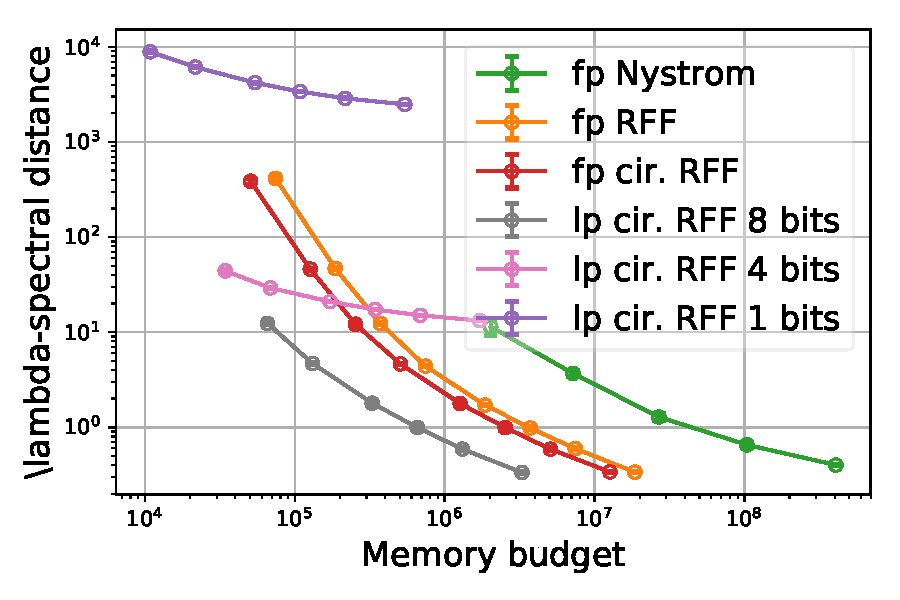
\includegraphics[width=0.33\linewidth]{figures/regression_delta_vs_mem.pdf} &
		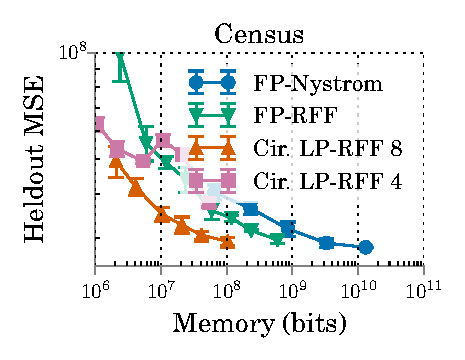
\includegraphics[width=0.33\linewidth]{figures/regression_l2_vs_mem.pdf} &
		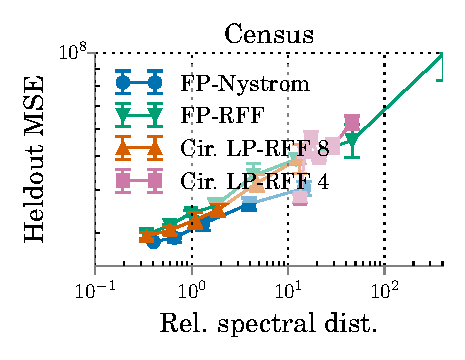
\includegraphics[width=0.33\linewidth]{figures/regression_l2_vs_delta.pdf} \\
		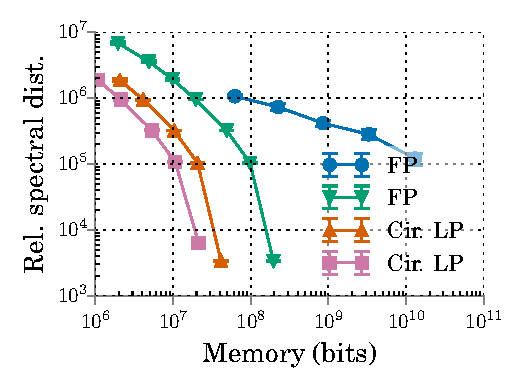
\includegraphics[width=0.33\linewidth]{figures/classification_delta_vs_mem.pdf} &
		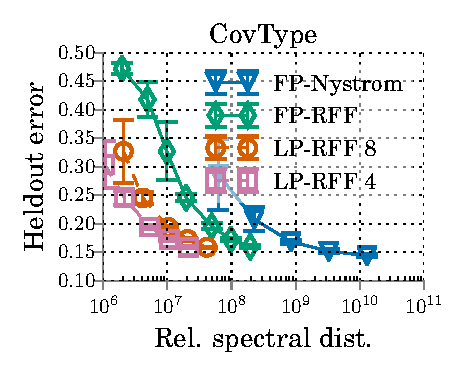
\includegraphics[width=0.33\linewidth]{figures/classification_acc_vs_mem.pdf} &
		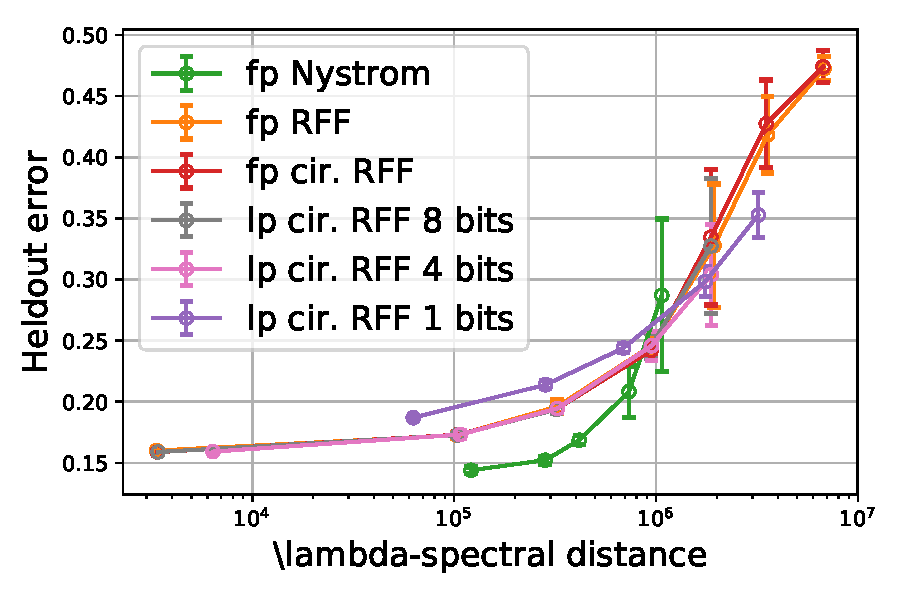
\includegraphics[width=0.33\linewidth]{figures/classification_acc_vs_delta.pdf} \\
		(a) & (b) & (c)
	\end{tabular}
	\caption{The strong correlation between generalization performance and $\lambda$-spectral distance $D_{\lambda}(K,\tK)$ under memory budgets for the Census dataset (top) and subsampled CovType dataset (bottom). Under different memory budget in (a) and (b), the precision demonstrates smaller $D_{\lambda}(K,\tK)$ tends to have better generalization performance. In (c), different kernel approximation approaches demonstrate similar generalization performance for similar $\lambda$-spectral distance.}
	\label{fig:specdist}
\end{figure}

